\documentclass[twocolumn]{htl-author}

\DOI{2012.0357}

\begin{document}

\title{The title of this paper is a contribution to the healthcare technology field}

\author{Haogang Ding$^{1}$, John S. Smith$^{2}$ and Maria Pascal$^{2}$}

\address{$^{1}$Laboratory for Life Sciences Engineering, Shanghai University, Shanghai, 200240, People's Republic of China\\
E-mail: Hding1963@shanghai.edu\\
$^{2}$Department of Biomedical Engineering, London University, Old Bridge Road, London, SW1 2AE, UK}

\historydate{Published in Healthcare Technology Letters; Received on xxx; Revised on xxx}

\abstract{The abstract should be no more than 200 words. Neural signal propagation is completely different from electron transport in conventional electronic devices. The electrical control of propagation of neural signal in a single neuron is interesting in neural device application in future, which could be the base of the future pain control or activation of neuron in a part of body. A new dimension to integrated circuits technology for lab-on-a-chip systems by employing 3D integration for improved performance and functionality is presented. It is proposed that a disposable biosensing layer can be aligned and temporarily attached to the 3D CMOS stack by the vertical interconnections, and can be replaced after each measurement.}

\maketitle

\section{Introduction}
Source localisation using electroencephalography (EEG) is to estimate the electrical activity of sources in the brain from the measurements of electric potential on the scalp. In general, source localisation error is due to modeling errors and measurement noise. Although several studies \cite{1,2} have suggested de-noising techniques, there is a limit to reduce noise from measurement data due to the nature of EEG and unavoidable internal/external noises. A subject-dependent model with exact conductivity values and sensor locations allows us to have a forward solver with a small source localisation error \cite{3}. However, the process
generating the computational model with a higher density and complexity by MRI or CT takes much time and huge effort, and we need more time to perform forward computations using the generating model. Nowadays,
a single-trial analysis or brain computer interface demands a real-time process, so EEG measurements with a low signal-to-noise ratio (SNR) are necessarily used for such purpose \cite{4}. Since the localisation errors due to the uncontrolled noise remain regardless of the model, it is not efficient to take an effort to obtain complicated model. Thus, the in-depth study for the relation between noise level and the complexity of the model is required. In this study, we investigated the source localisation effects of realistic human head model with various geometrical deformations particularly for a set of low SNR EEG measurements. In order to evaluate implicit modelling errors due to geometrical deformation, the seven realistic head models decomposed by tetrahedral elements were constructed from the same MRI data set.


\section{Analytical modelling}
This approach combines the advantages of both active-electronic and passive-electronic (disposable) biochips in one system. The top sensing layer is temporarily attached to the analogue interface circuit through vertical interconnections. These allow the fabrication of high density multi-target arrays since they solve the horizontal signal routing problem encountered in disposable biosensors \cite{5}. In addition, since the interface electronics is in the direct neighbourhood of the array, weak sensor-signals can be amplified while being minimally affected by the parasitic effects, thus leading to considerable improvement in the sensitivity and the signal integrity. Analogue outputs are converted to digital signals through on-chip ADC converters and processed by dedicated digital electronics. Hence, the signal processing required to solve complex algorithms for target identification can be accomplished on the system. Fig. \ref{fig1} Shows a typical output. This technology also allows employing different measurement techniques (cyclic voltammetry, impedance measurement, etc.) by simply replacing the top sensing layer and configuring the analogue front-end accordingly.

\begin{figure}[!h]\label{fig1}
\centering{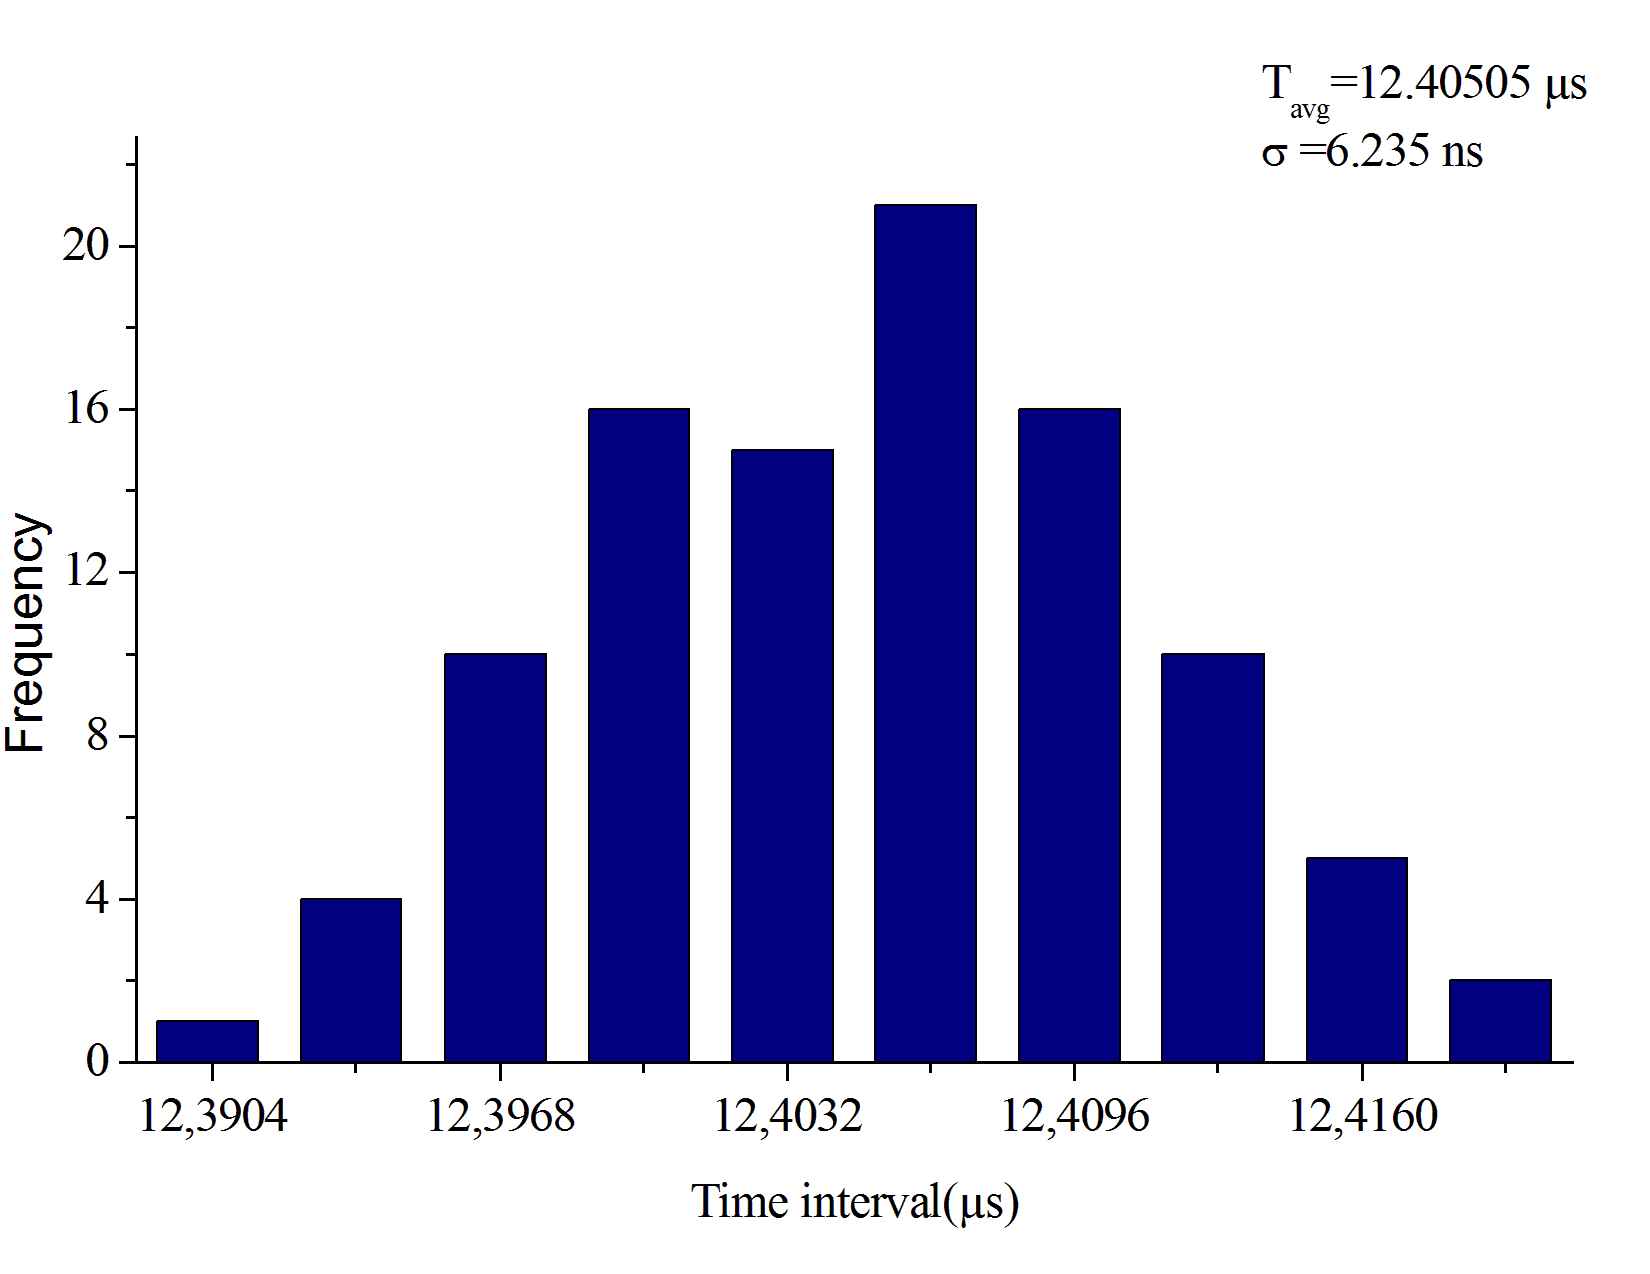
\includegraphics[width=8cm]{fig1.pdf}}
\caption{Frequency histogram}
\end{figure}

\begin{center}
\begin{table}[!b]%[width=7cm, height=8cm]
\caption{Summary of many of the capsule devices.}
\scalebox{0.55}{
\begin{tabular}{|l|l|c|}
  \hline
  % after \\: \hline or \cline{col1-col2} \cline{col3-col4} ...
  \textbf{Device} & \textbf{Descriptions} & \textbf{Measurement} \\\hline
  SMART pill \cite{6} & Intra-luminal pH measurement, tubeless gastric analysis, an & Pressure, pH \\
  & alternative for pentagastrin tests & \\\hline
  M2A \cite{7} & Imaging within GI tract, positive for the inspection of IBDs and & Image \\
  & Crohn's disease.  & \\\hline
  NASA pill \cite{8} & Core-body temperature measurement, identify temperature & Temperature, pressure \\
  & changes within a potentially ulcerated area.   & \\\hline
  BRAVO \cite{9} & Catheter-free oesophageal pH monitoring, GERD diagnosis & pH \\\hline
  InteliSite \cite{10} & Assessing drugs absorption within a specific region of the GI  & N / A \\
  & tract.   & \\\hline
  GI micro-robot  & Bi-directional wireless endoscopes with real-time imaging and  & Image \\
  \cite{11}& process.   & \\\hline
  MMM \cite{12} & Magnetic markers as a non-invasive tool to monitor GI transit & Location \\\hline
  Inchworm \cite{13} & Semi-mechanic device can be externally controlled for in-gut localisation & N / A \\
   & localisation.   & \\\hline
  Medical & Capsule-shaped magnetic actuator and capsule micro pump can  & N / A \\
   actuator \cite{14}   & be used inside GI tract.   & \\\hline
  IDEAS \cite{14} & Bringing together System-on-Chip and Lab-on-a-Chip  & Temperature,  \\
      & methodologies to develop a GI monitoring microsystem. & conductivity, pH,\\
     &  & dissolved oxygen  \\\hline
  Olympus \cite{14} & Wireless endoscope & Image \\
  \hline
\end{tabular}}
\end{table}
\end{center}
The fact that an ISFET is implemented on a simple planar substrate was exploited to microfabricate additional sensors on to the same chip.  The advantage of this approach was that it enabled multisensory functionality in the one device without the difficulties of adding more sensor components.  The device incorporated pH, temperature, conductivity and pO2 sensors into a single wireless capsule.  In this manner, packaging complexity and size was reduced. Despite integration of several sensors, the device still relied on a separate application specific integrated circuit to carry out electronic functions of sensor signal capture, data conversion and encoding for wireless transmission.  Because two chips are required with considerable chip-to-chip interconnect, space is used for little reward in the capsule. Notwithstanding the impact on size, a system based on a device that relies on a modified MOSFET is not suitable to mass manufacture.  Ideally, devices should be made exclusively using a conventional complementary metal oxide semiconductor (CMOS) process so that both sensors and the electronics can be co-integrated into a sensing system on a chip (SSOC).


\section{Method}
In the conversion phase, the time interval while the amplifier output voltage discharges until it reaches the threshold voltage of the comparator will be digitized by a counter. The equivalent temporal jitter is the amplifier output noise divided by the discharging slope as shown in the following equation:
\begin{equation}\label{equation4}
T_{jitter,RMS}=V_{out,RMS}\left( \dfrac{C_{h}}{I_{discharge}}\right)
\end{equation}
For 8ENOB$_{6\sigma}$ accuracy, the RMS jitter on a total conversion time range of 12$\mu$s
should be smaller than 7.8ns. For $I_{discharge}$ = 750nA, and $C_{h}$ = 20pF, this corresponds to a maximum acceptable RMS output noise voltage of 292.5 $\mu$V.

\begin{figure}[!b]
\centering{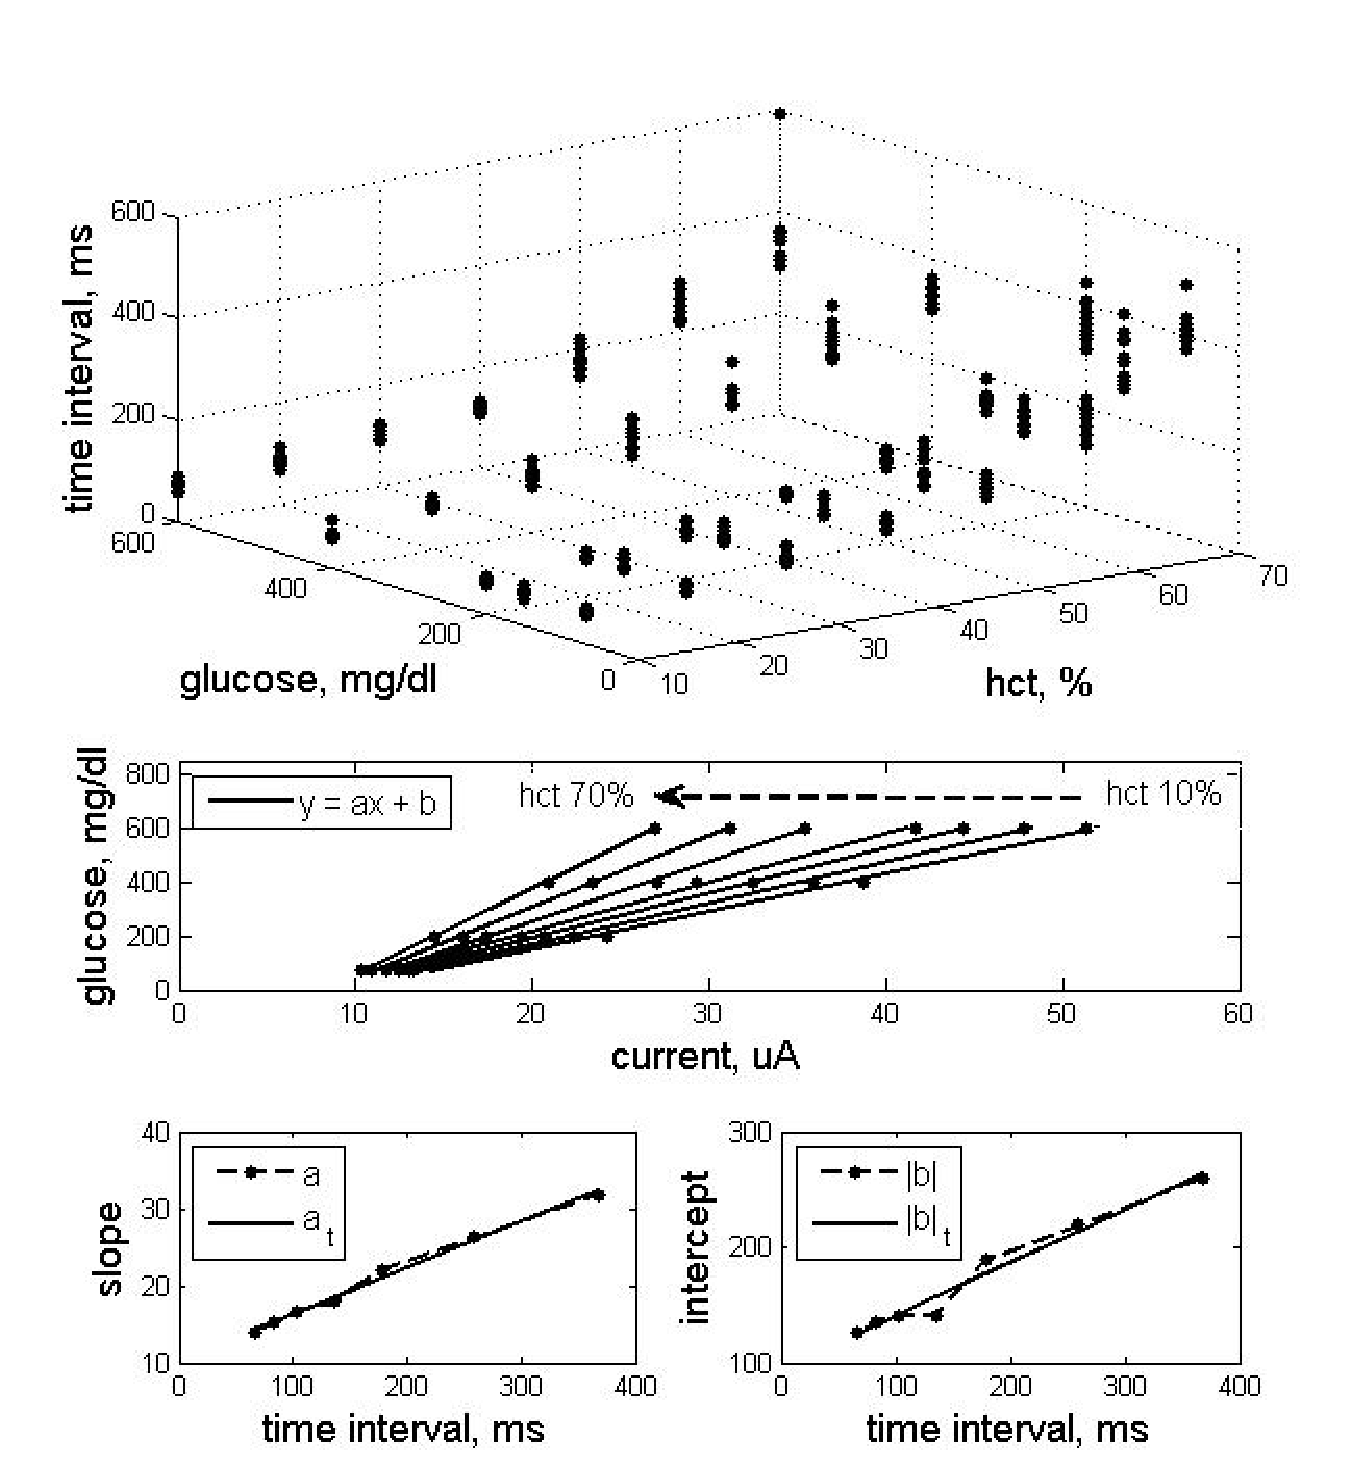
\includegraphics[width=8cm]{fig2.pdf}}
\caption{Estimation of glucose concentration by the adaptive calibration curve.}
\source{
\begin{flushleft}
a  Time interval detected between the working and third electrodes
b  Calibration curves in the HCT at 10, 20, 30, 40, 50, 60, and 70\%
c  Estimation of a (slope) for time interval in y=ax+b
d  Estimation of |b| (intercept) for time interval in  y=ax+b
\end{flushleft}}
\end{figure}

The main sources of noise at the amplifier output are the noise contribution of the amplifier itself ($V_{n_amp,RMS}^{2}=\frac{4kT}{3}\;\frac{1+C_1/C_2}{C_{c}}$ \cite{Schreier_Silva_Steensgaard_Temes05} where $C_{c}$ is the frequency compensating capacitor in the two-stage OA) and kTC noise of the two capacitors $C_1$ and $C_2$ ($V_{n,RMS}^{2}=\frac{kT}{C_{1}+C_{2}}$ at the sampling phase where k is Boltzmann constant, T is absolute temperature in degrees Kelvin). At the start of the amplifying phase, the total noise charge power across the two capacitors $Q_{n,1}^{2} = V_{n,RMS}^{2}{(C_1+C_2)^{2}}$ transfers to the capacitor $C_2$. By way of the feedback loop, the switch thermal noise on $C_1$ is transferred to $C_2$, contributing $\frac{kT}{C_1}\left(\frac{C_1}{C_2}\right)^{2}$ to the output noise in addition to the switch thermal noise on $C_2$ itself. All kTC noise summed up is:
\begin{equation}
V_{n,RMS}^{2}=\dfrac{kT}{C_{1}+C_{2}}\left(\dfrac{C_1+C_2}{C_2}\right)^{2}+\frac{kT}{C_1}\left(\frac{C_1}{C_2}\right)^{2}+\dfrac{kT}{C_2}
\label{equation2}
\end{equation}
Thus, with the gain $C_1/C_2 =15$, and adding the amplifier noise the total output noise power is:
\begin{equation}
V_{out,RMS}^{2} = 32\dfrac{kT}{C_{2}}+\dfrac{64}{3}\dfrac{kT}{C_c}\\
\label{equation3}
\end{equation}
With $C_{c}$= 4pF, the minimum value for $C_2$ is 2.67pF. To allow for some margin, $C_{2}$=4pF and consequently $C_1$=60pF have been chosen.




\section{Results}
Fig.3 (a) shows a schematic diagram of the three terminals measurement system. The control electrode was inserted between the stimulation electrode and the measurement electrode with a negative applied voltage of -400 mV. In this case the distance between electrodes is 120 ?m. Fig. 3(b) shows a top view observed by an optical microscope. In this picture, spare electrodes just beside each electrode are also shown but are not used in this experiment. As shown in this optical microscope, neuron is bridged through three electrodes; stimulation, control and measurement electrode.
Fig.3(c) shows a typical active potential observed at the measurement electrode as a function of time gap between the voltage applied to the stimulated electrode and that to the control electrode. On the first electrode, that is, the stimulation electrode, a proper voltage of about 400mV is applied to stimulate the neuron and to generate the active potential. We have already confirmed that this active potential excited at the stimulation electrode propagates through the neuron in the two electrodes experiment mentioned above. When we applied the voltage of -400mV on the control electrode with some timing of less than 26?sec, it is found the active potential at the measurement electrode is about 10mV and is strongly suppressed compared to the active potential of 80 mV without applying the voltage on the control gate (in this system, the active potential is 80mV). Beyond 26 ? sec the active potential became 80mV because the neural signal has passed away the control gate and no influence remains on the neural signal transport. Therefore, to suppress the propagating signal by the control electrode the timing of the voltage applied to the control electrode relative to the applied voltage on the stimulation electrode is very important.


\begin{figure}[!t]
\centering{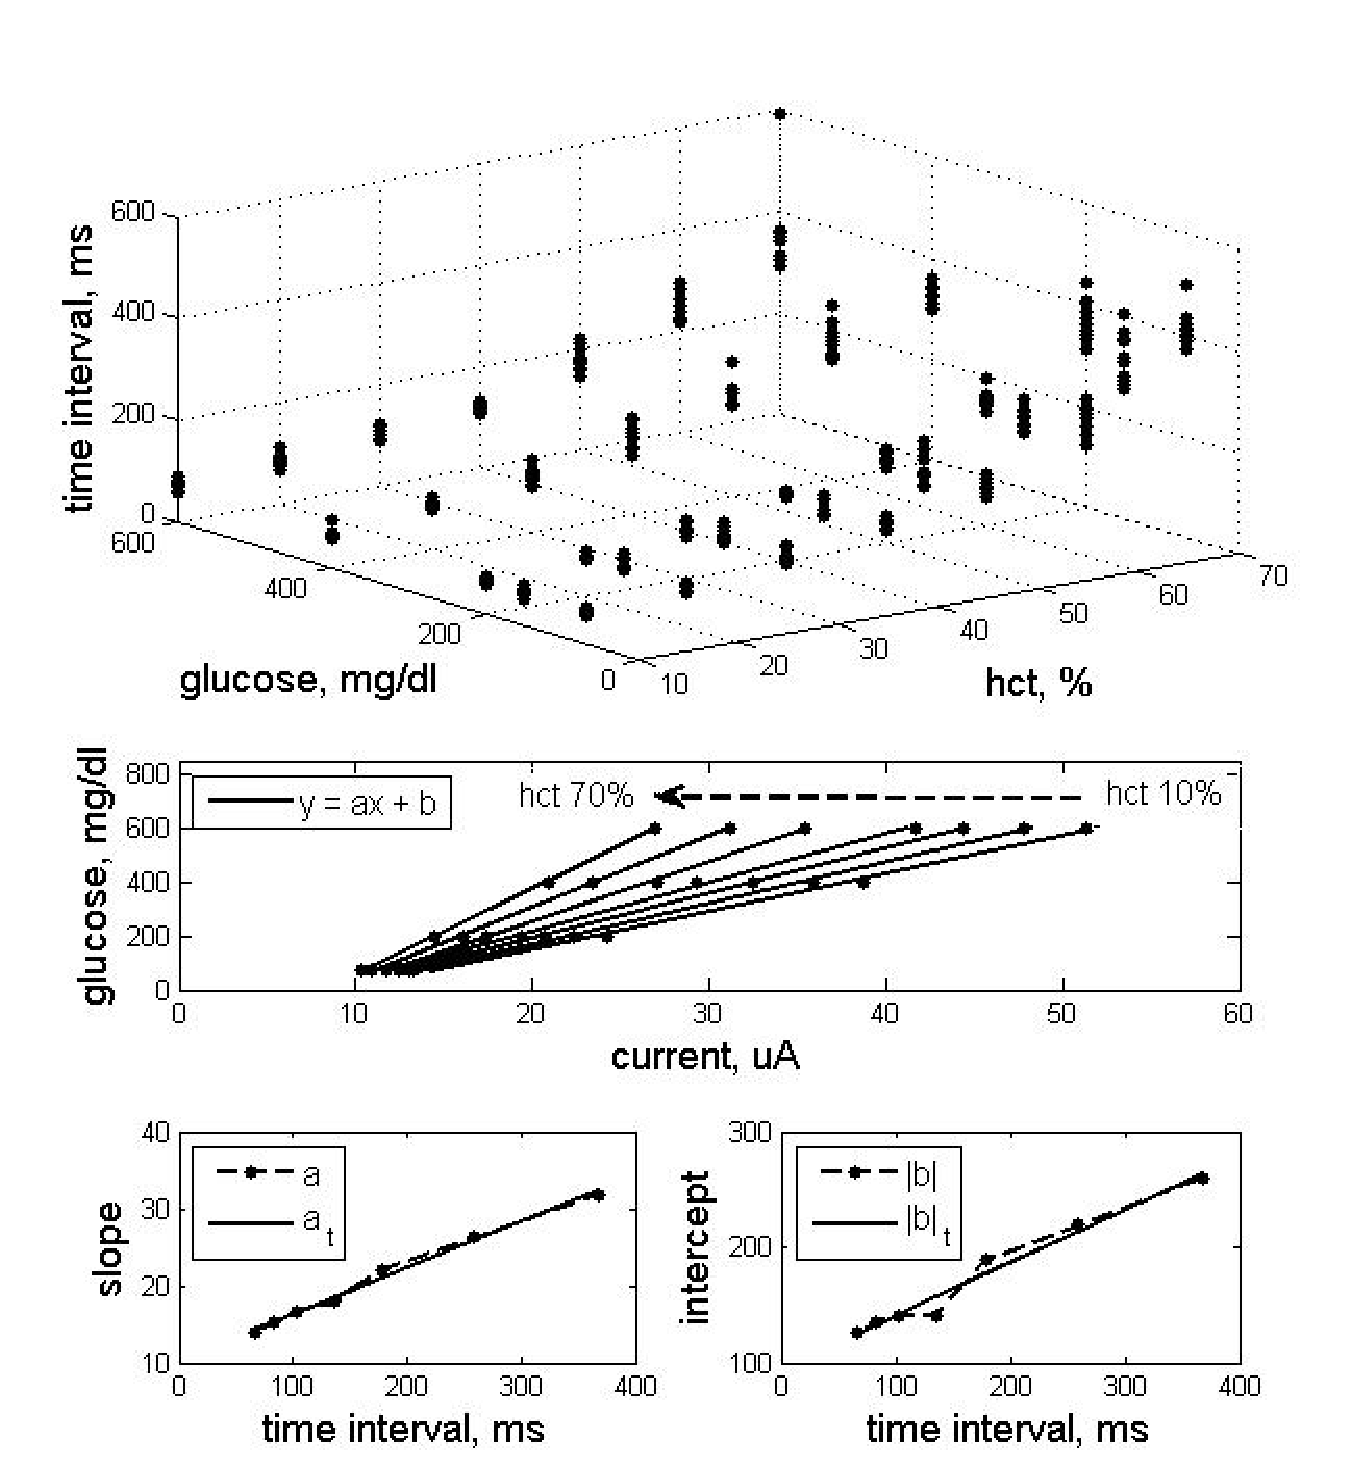
\includegraphics[width=8cm]{fig2.pdf}}
\caption{The three terminals measurement system and a typical active potential}
\source{
\begin{flushleft}
\footnotesize{a  schematic diagram of the three terminals measurement system
b  top view observed by an optical microscope
c  typical active potential}
\end{flushleft}
}
\end{figure}


\section{Conclusions}
The proposed inhibitory mechanism is physiologically based on the electrical stimulation of the mental nerve with a low current and high frequency stimulus. The afferent responses that are generated are directed towards higher nervous centers (brain stem). These afferent signals are processed by neurons that inhibit (decrease) motor responses for the contraction of muscles involved in the elevation of the jaw.

When stimulated with high frequencies, the threshold of stimulus perception increases, making the subject perceive less electrical current. This helps the patient not to notice the stimulation while sleeping.

The decreased activity measured in the mandibular elevator muscles indicate that inhibition responses can be generated. Therefore, this method is a good starting point for possible future use in patients with SB. Future work involves testing during bruxism episodes while sleeping. Results shown that is necessary to develop a new electronic stimulator capable of stimulate in these range of frequency, amplitude and pulse width values.


\ack{The work described in this paper was funded by the TRYH Biomedical Research Centre Programme. Dr John Smith is supported by the Wellcome Trust and EPSRC under grant number PW 089871/Z/06/P.}

\begin{thebibliography}{14}

\bibitem{1} 1  Rao, L.V., Jakubiak, F., Sidwell, J.S., Winkelman, J.W., Snyder, M.L.: 'Accuracy evaluation of a new glucometer with automated hematocrit measurement and correction', \textit{Clinica Chimica Acta.}, 2005, {\bf 356}, pp. 178-183

\bibitem{2} Tang, Z., Lee, J.H., Louie, R.F., Kost, G.J.: 'Effects of different hematocrit levels on glucose measurements with handheld meters for point-of-care testing'. \emph{Arch Pathol Lab Med.}, 2000, {\bf 124}, pp. 1135--1140

\bibitem{3} 3  Secomski, W., Nowicki, A., Tortoli, P., Olszewski, R.: 'Multigate doppler measurements of ultrasonic attenuation and blood hematocrit in human arteries', \emph{Ultrasound in Medicine and Biology}, 2009, {\bf35}, pp. 230--236

\bibitem{4} Cinar, Y., Demir, G., Pac, M., Cinar, A.B.: 'Effect of hematocrit on blood pressure via hyperviscosity', \emph{American Journal of Hypertension}, 1999, \textbf{12}, pp. 739-743

\bibitem{5}Mackenzie, M.R., Lee, T.K.: 'Blood viscosity in waldenstrom's macroglobulinemia', \emph{Blood}, 1974, \textbf{44}, pp. 87--98

\bibitem{6} Hendriks, B.H., Bierhoff, W.C.J., Horikx, J.J.L., Desjardins, A.E., Hezemans, C.A., 't Hooft, G.W., Lucassen, G.W., and Mihajlovic, N.: 'High-resolution resonant and nonresonant fiber-scanning confocal microscope', \emph{J. Biomed.Opt.}, 2011, \textbf{16}(2), 026007

\bibitem{7} Wall, R.A., Bonnema, G.T., and Barton, J.K.: 'Novel focused OCT-LIF endoscope', \emph{Biomed. Opt. Express}, 2011 \textbf{2(3)}, 421--43

\bibitem{8} Li, E., Peng, G.-D., and Ding, X.: 'High spatial resolution fiber-optic Fizeau interferometric strain sensor based on an in-fiber spherical microcavity', \emph{Appl. Phys. Lett.}, 2008, \textbf{92}, 101117

\bibitem{9} Mao, Y., Flueraru, C., Chang, S., Popescu, D.P., and Sowa, M.G.: 'Performance analysis of a swept-source optical coherence tomography system with a quadrature interferometer and optical amplification', \emph{Opt. Commun.}, 2011, \textbf{284}, pp. 2622--2627

\bibitem{10}Kajihara, Y., Fukuzawa, K., Itoh, S., and Zhang, H.: 'Real-time visualization of a shearing nanometer-thick lubricant film by two-stage imaging ellipsometric microscopy', IEEE Trans. Magnet., 2011, \textbf{47}(10), pp. 3441-3444

%\vfill\pagebreak

\bibitem{11} Pedrotti, F.L., Pedrotti, L.M., and Pedrotti, L.S.: 'Introduction to Optics' (Pearson Addison Wesley, San Fransisco, CA, 2007)

\bibitem{12} Lorenser, D., Yang, X., Kirk, R.W., Quirk, B.C., McLaughlin, R.A., and Sampson, D.D.: 'Ultrathin side-viewing needle probe for optical coherence tomography', \emph{Opt. Lett.}, 2011, \textbf{36}(19), pp. 3894--3896

\bibitem{13} Ryu, S.Y., Choi, H.Y., Na, J., Choi, W.J., and Lee, B.H.: 'Lensed fiber probes designed as an alternative to bulk probes in optical coherence tomography', \emph{Appl. Opt}., 2008, 47(10), pp. 1510--1516

\bibitem{14} 14  Han J.-H., and Kang, J.U.: 'Microball lens integrated fiber probe for optical frequency domain imaging', \emph{Chin. Opt. Lett.}, 2011, \textbf{9}(9), 090608

\end{thebibliography}

\end{document}
